\documentclass[12pt]{article}
\usepackage[utf8]{inputenc}
\usepackage{style}

\title{Oracle Quantum Computing}
\author{Joshua Spayd}
\date{\today}

\begin{document}
\maketitle

\section{Introduction}
It is the objective of the theoretical sciences to develop mathematical models
that describe natural phenomena, and when faced with a result that contradicts
existing models, it is the responsibility of the theorist to augment these
models to reconcile with the observed phenomena, and to resolve
inconsistencies across scientific theories. The strong Church-Turing thesis
conjectures that every physically realizable computation model can be
simulated by a Turing machine with polynomial overhead in runtime, but
physicist Richard Feynman \cite{Fey82} notes that the obvious classical
algorithm for simulating a quantum system of $n$ particles runs exponentially
in $n$ and suggests that computers be equipped with quantum mechanical gates
in order to enable efficient simulation of quantum systems. If quantum systems
cannot be efficiently simulated by Turing machines --- and if general-purpose
quantum computers are physically realizable --- then the strong Church-Turing
thesis is false, and we require a new model of computation. Though questions
of the feasibility and relative efficiency of quantum computers are yet
unanswered, this uncertainty has not prevented theorists from developing
quantum computational models. In this paper, we will formalize quantum computing
and quantum oracles, and then we will describe a few results from quantum
complexity theory, with emphasis on the result from \cite{BB92} that relative to
certain oracles, quantum computers are more powerful than nondeterministic
computers, or in the words of  Berthiaume and Brassard, that ``quantum can beat
nondeterminism.''


\section{Quantum superposition: the two-slit experiment}
Before we attempt to formalize quantum computation, it will help to understand
the physical ideas behind such a formalization. To illustrate these principles,
we turn to the two-slit experiment. In the two-slit experiment, a photon source
id placed on one side of a wall that has two slits in it. On the other side is
an array of detectors that light up when hit by a photon. Consider the rate at
which photons hit these detectors. If one slit is covered, we might expect that
the detector behind the open slit will receive the highest rate of photons per
hour, which is indeed what happens, as depicted in \cref{fig:two-slit-1}.

\begin{figure}[H]
  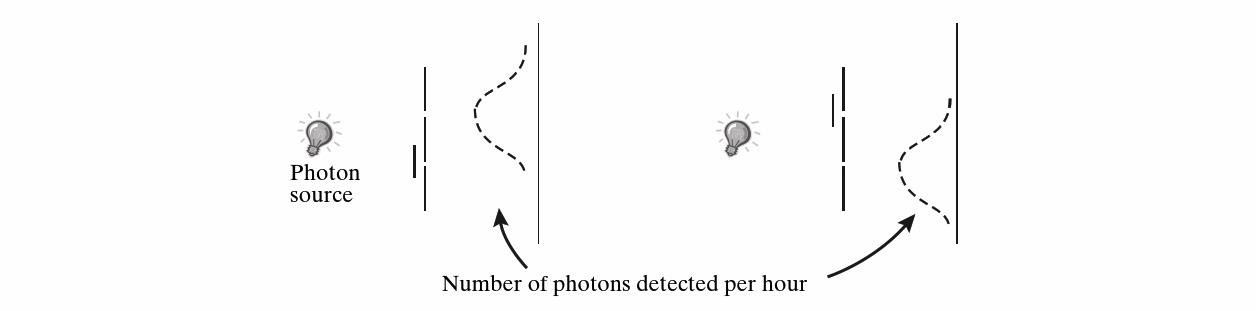
\includegraphics[width=\textwidth]{two-slit-1}
  \caption{\cite[p. 203]{AB09}}
  \label{fig:two-slit-1}
\end{figure}

If we uncover both slits, then we may expect that a detector will receive a rate
of photons equal to the sum of the rates it receives when one of each of the
slits is covered, but this is not what happens. In fact, as depicted in
\cref{fig:two-slit-2}, some detectors even receive a lower rate of photons than
this sum.

\begin{figure}[H]
  
\includegraphics[width=\textwidth]{two-slit-2}
  \caption{\cite[p. 203]{AB09}}
  \label{fig:two-slit-2}
\end{figure}

This phenomenon can only be explained by quantum mechanics. When a photon leaves
the photon source, it does not follow a single path to some detector; rather, it
instantaneously explores all possible paths, where each path has some associated
\emph{amplitude}, which may be positive or negative (or zero). If two paths
arrive at the same detector with opposite signs, then they cancel-out, or
\emph{interfere}. However, perhaps we are skeptical of this all-paths
exploration, and we decide to add detectors at each slit that light up when a
photon passes through the slit. If photons are truly exploring all possible
paths, then we might expect to measure some of the same photons at both slits.
But now that we are measuring the photons at the slits, we instead see what we
originally expected: each detector receives a rate of photons equal to the
sum of the rates of photons it receives when one of each of the slits is
covered. This experiment gives us an idea of both some of the strengths and
weaknesses of quantum computers: if we can in some sense ``explore all paths,''
then we may be able to simulate nondeterminism efficiently, but the nature of
our quantum parallelism must play nicely with quantum interference, and once we
measure a result, we lose any parallelism that we may have.


\section{Modeling quantum computation}
We begin our model with a description of memory. On a classical computer, we
normally model memory as a sequence of bits, each of which can be 0 or 1. In
our model of quantum computers, the smallest piece of memory is the
\emph{qubit}, which can take on the basic states $\qz$ and $\qo$, or may also be
in a \emph{superposition} of these states of the form
$$
  \alpha_0\qz + \alpha_1\qo,
$$
where $\alpha_0, \alpha_1 \in \CC$ are \emph{amplitudes} satisfying
$\abs*{\alpha_0}^2 + \abs*{\alpha_1}^2 = 1$.\footnote{Recall that for a complex
number $z = a + bi$ where $i=\sqrt{-1}$, we have $\abs*{z} = \sqrt{a^2+b^2}$.}
When we observe the qubit, it is revealed to be in state $\qz$ with probability
$\abs*{\alpha_0}^2$ and state $\qo$ with probability $\abs*{\alpha_1}^2$. Once
the qubit is measured, its amplitude wave \emph{collapses}, and the values of
its amplitudes are lost. Our state of memory, then, is an $m$-qubit register
$\reg*{b_1, b_2, \dots, b_m}$ described by a superposition of the form
$$
  \alpha_{0\dots 0}\reg*{0\dots 0}
  + \alpha_{0\dots 1}\reg*{0\dots 1}
  + \dots
  + \alpha_{1\dots 1} \reg*{1\dots 1},
$$
where $\sum_{x \in \zo^m} \abs*{\alpha_x}^2 = 1$. When the system is observed,
it is revealed to be in state $\reg*{x}$ with probability $\abs*{\alpha_x}^2$
for each $x \in \zo^m$. We will sometimes denote the state $\reg*{xy}$ as
$\reg*{x}\reg*{y}$.

\subsection{Quantum operations}
\begin{defn}[Quantum operation {\cite[p. 210]{AB09}}]
  \label{defn:op}
  A \emph{quantum operation} for an $m$-qubit register is a funciton $F :
  \CC^{2^m} \to \CC^{2^m}$ that maps its previous state to the new state and
  satisfies the following conditions:
  \begin{adjustwidth}{0.25in}{0in}
    \emph{Linearity:} $F$ is a linear function. That is, for every $\vec{v} \in
    \CC^{2^n}$, $F(\vec{v}) = \sum_x \vec{v}_x F(\reg*{x})$. \\
    \emph{Norm preservation:} $F$ maps unit vectors to unit vectors. That is,
    for every $\vec{v}$ with $\norm*{\vec{v}}_2=1$, $\norm*{F(\vec{v})}_2=1$.
  \end{adjustwidth}
\end{defn}

\subsection{Quantum Turing machines and the class $\BQP$}
\begin{defn}[Quantum computation and the class $\BQP$ {\cite[p. 213]{AB09}}]
  \label{defn:bqp}
  Let $f : \zo^* \to \zo$ and $T : \NN \to \NN$ be some functions. We say that
  $f$ is \emph{computable in quantum $T(n)$-time} if there is a polynomial-time
  classical TM that on input $\paren*{1^n, 1^{T(n)}}$ for any $n \in \NN$
  outputs the descriptions of quantum gates $F_1, \dots, F_T$ such that for
  every $x\in \zo^n$, we can compute $f(x)$ with probability at least
  $\nfrac{2}{3}$ by the following process:
  \begin{enumerate}
    \item Initialize an $m$-qubit quantum register to the state
      $\reg*{x0^{n-m}}$ (i.e., $x$ padded with zeroes), where $m \le T(n)$.
    \item Apply ons after the other $T(n)$ elementary quantum operations $F_1,
      \dots, F_T$ to the register.
    \item Measure the register and let $Y$ denote the obtained value. (That is,
      if $\vec{v}$ is the final state of the register, then $Y$ is a random
      variable that takes the value $y$ with probability $\abs*{\vec{v}_y}^2$
      for every $y \in \zo^m$.)
    \item Output $Y_1$.
  \end{enumerate}
  A Boolean function $F : \zo^* \to \zo$ is in $\BQP$ if there is some
  polynomial $p : \NN \to \NN$ such that $f$ is computable in quantum
  $p(n)$-time.
\end{defn}

\begin{thm}
  $\BPP \subseteq \BQP$.
\end{thm}

\begin{thm}
  $\BQP \subseteq \PSPACE$.
\end{thm}

\begin{conj}
  $\NP \not\subseteq \BQP$.
\end{conj}

\begin{thm}[\cite{BBBV97}]
  Relative to an oracle chosen uniformy at random, with probability 1, the class
  $\NP$ cannot be solved on a quantum Turing machine in time $\smallo{2^{n/2}}$.
\end{thm}
``There is no black-box approach to solving $\NP$-complete problems using some
uniquely quantum features of QTMs.''

\begin{conj}
  $\BPP \subsetneq \BQP$.
\end{conj}

\begin{thm}[\cite{Sho97}]
  $\lang{Factoring} \in \BQP$.
\end{thm}

\begin{thm}[\cite{BB92}]
  Under appropriate oracles, there is a decision problem that can be solved in
  polynomial time on a quantum computer that would require exponential time on a
  classical nondeterministic computer.
\end{thm}
``Quantum can beat nondeterminism.''

\section{Quantum oracles}
\TODO{Refer to {\cite{BBBV97}}.}


\section{Quantum can beat nondeterminism \cite{BB92}}


\nocite{*}
\bibliographystyle{alpha}
\bibliography{bibliography}
\end{document}
